\newpage
%In the drone
\subsection{Conductivity}
Conductivity of a substance is defined as 'the ability or power to conduct or transmit heat, electricity, or sound'. \cite{merriamconductivity} Its units are Siemens per meter [S/m] in SI. Electrical conductivity is defined as the ratio between the current density (J) and the electric field intensity (e) and it is the reciprocal of the resistance:

\[s = J/e = 1/r\]

In water and ionic materials or fluids a net motion of charged ions can occur. This phenomenon produce an electric current and is called ionic conduction. Pure water is not a good conductor of electricity. Because the electrical current is transported by the ions in solution, the conductivity increases as the concentration of ions increases. \cite{lenntech} Conductance in water also depend on the mobility of the ions, the valence, and the temperature of the substance. \cite{standardmethods}\\


\subsubsection{Salinity}
In natural water, salinity is often determined by measuring the conductivity of the water. Typical values go as follows:

\begin{figure}[h]
\centering
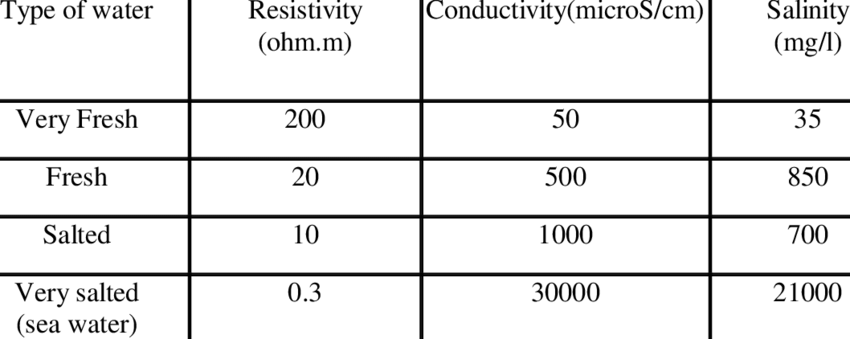
\includegraphics[scale=0.4]{water/61_typicalvalues.png}
\caption{Typical resistivity, conductivity and salinity values for different types of water \cite{abdulsamsudin}}
\end{figure}

\newpage
\subsubsection{Sensors}
In this section, a comparison between potential conductivity sensors for the project is given. Certain features like price, accuracy, and form factor will be given.

To ensure accuracy, a conductivity probe needs to be calibrated first in two buffer solutions of 1413us/cm and 12.88ms/cm. \cite{DFR0300H} This has to be done every month. These buffer solutions usually cost around €13,- or can be found in most chemistry labs.

\paragraph{Analog Devices EVAL-CN0349-PMDZ}\mbox{€49,04} \cite{CN0349}
\begin{table}[h!]
	\centering
	\adjustimage{height=4cm,valign=c}{water/62_cn0349.jpg}\quad
	\begin{tabular}{| l | l |}
    \hline
    Protocol & I2C\\
    Measurement Accuracy &  1\% FSR\\
    Supply Voltage & 3.3V\\
    Software library included & no \\
    Probe included & yes \\
    Availability & 2 Months \\
    \hline
	\end{tabular}
\end{table}

\paragraph{Gravity: Analog Electrical Conductivity Sensor}\mbox{€72,70} \cite{DFR0300H}
\begin{table}[h!]
	\centering
	\adjustimage{height=4cm,valign=c}{water/63_dfr0300h.jpg}\quad
	\begin{tabular}{| l | l |}
    \hline
    Protocol & Analog\\
    Measurement Accuracy &  5\% FSR\\
    Supply Voltage & 3.3-5V\\
    Support Detection Range & 10~100ms/cm\\
    Software library included & yes \\
    Probe included & yes \\
    Availability & 3-5 Working days \\
    \hline
	\end{tabular}
\end{table}